\section{Method \& apparatus}
\label{method}
Past research has shown that both rapid serial visual presentation (RSVP) and neurofeedback (NF) have positive effects on reading and concentration. Our approach posits that a RSVP controlled by self-regulated neurofeedback may help build a new kind of brain-computer interface (BCI), which would allow people read fast, yet at their own pace, and at the same time, maintain engagement. Thus readers can avoid multitasking, and keep concentrated on reading (e.g., a long newspaper article).

We hypothesize that meaningful brain wave modulations can be extracted from EEG recordings obtained from even the simplest consumer-grade brain scanner. This signal is then used to update the rate of RSVP in real-time. The updated RSVP rate in turns influences brain wave modulations (see Figure \ref{fig:apparatus}). The influence loop between the brain (i.e., wave modulations) and the computer (i.e., RSVP rate) variables constitute a feed-back loop, which is a typical neurofeedback feature. If the RSVP rate stabilizes, then self-regulation is achieved. On the contrary, if the rate drifts away (i.e., slower or faster rate), then a positive (resp. negative) feedback loop occurs: This is a signature of failure to self-regulate, and thus, to effectively synchronize with the task at hand. Our main aim here is precisely to determine how well users actually achieve self-regulation, and how it influences their speed reading experience, including comprehension and recall.

Our approach is novel in a number of ways, and thus, carries as many technical challenges. Most BCIs involve having a specific mental gesture (see e.g., \cite{chuang2013ithink,jonhson2014mythoughts}) or a stimulus (e.g., \cite{}) elicit a corresponding response by the computer. This approach requires some training by the user to repeat the gesture and/or for the computer to recognize the mental state associated with a stimulus. On the contrary, with the {\it brain speed reader} the ordered sequence of stimuli (i.e., words) triggers small incremental reactions and rate changes, as a result of learning {\it on the fly} and control through self-regulation.

\subsection{Avoiding ``under-control"}
The main challenge for such novel BCI lies in the capability to process information from EEG recordings at a speed in adequacy with the RSVP rate, in order to avoid ``under-control": On the contrary to over-control,\footnote{A typical example of over-control is when it takes several minutes (resp. hours) for the heating system of a house to adjust the temperature in a room after a quick thermostat adjustment by the operator. The operator may be tempted to adjust too often or too much to compensate the slow temperature change, thus leading to huge temperature amplitudes, or even resonance phenomena.} if acquiring, processing information, and taking a control decision takes more time than the evolution pace of the state variable (i.e., here, the RSVP rate), then control action is always behind and thus inefficient. Molly Potter, one the pioneers of cognitive science using RSVP, pointed out early that a control in real-time of the RSVP presentation rate would be desirable, both for science and application purposes. However, she acknowledged that any mechanical means (e.g., through keystrokes, or eye-blinking) would take to much time and introduce too much delay in comparison with the presentation rate, hence leading to a form of under-control \cite{potter1984rapid}.

\subsection{Quality, processing \& usability tradeoffs}
Even if no mechanical input is involved and signal used for RSVP rate control is sourced directly from the brain, avoiding under-control is still a challenge: EEG signal is notoriously noisy, and signal quality and resolution improves significantly with the number and the quality of electrodes \cite{michel2004eeg}. Yet, each supplementary electrode requires additional processing time, which increase at best linearly, but most likely at the square of the number of electrodes, if correlations between EEG signals from electrodes exist, which is most often the case. There is thus a trade-off between input quality and processing time, taking into account that poor signal quality may require additional data cleaning and thus, processing time. The choice of recording technology influences qualitatively which approaches can be used to analyze EEG signal: For instance, low quality EEG equipment can hardly detect event-related potentials (ERPs), even if these ERPs are repeated multiple times to average out noise \cite{ERP_consumergrade_EEG}. The design choice is also constrained by time: The average RSVP rate is 125 milliseconds (ms) per word. EEG signal must therefore take less than 125 ms to process and deliver the next rate update, and the less processing time, the more the BCI is in sync with ``orders" provided by the brain. Finally, the more sophisticated the EEG recording device used, the less obvious and wearable the form factor. Hence, in the case of EEG, sophistication comes at the cost of usability, potential scaling limitation of the user base, and thus, limitation of social benefits of the brain speed reader.

\subsection{Entropy as an efficient way to compress the EEG signal}
Here, we operate and test the brain speed reader with the cheapest consumer-grade EEG headset available on the market, with one dry electrode placed on position {Fp1} in the 10--20 electrode system \cite{klem1999ten}. Namely, we try to elicit self-regulation with the simplest and most accessible EEG recording device (Neurosky Mindwave, approximative budget: \$100). The EEG signal recorded at 512 Hz is processed in the spectral domain: The Shannon entropy of the power spectrum of the last quarter second of EEG signal (128 measures) is computed as, 

\begin{equation}
\label{eq:shannon}
S = - \sum_{i=1}^n p_i\cdot log_{2}(p_i),
\end{equation}

with $p_i$ is the activity level of the i-est frequency between $0$ and $128$ Hz (resampled and normalized following \cite{merrill2015}). $S$ is then normalized into 

\begin{equation}
\label{eq:Snormalized}
S_{norm}(t) = \frac{S(t) - \langle S \rangle}{\sigma_{S}}, 
\end{equation}

with $\langle S \rangle$ and $\sigma_{S}$ the average and standard deviation of the entropy $S$ calculated over the last 5 seconds. $S_{norm}(t)$ ensures that only deviations of brain wave modulations from the average influence the RSVP rate. The measure of entropy is particularly handy because it {\it compresses} information contained in a whole density function into a scalar. Entropy is thus one simple and non-parametric way to account for the variation of power spectrum density function, given that the density function of brain wave frequencies is roughly pink noise, which follows a power law heavy-tailed density function given by $pdf(f) \sim 1/f^{\mu+1}$, with $f$ the frequency and $\mu \approx 1$. When working with the power spectrum of brain waves, researchers tend to dismiss frequencies higher than 60Hz, because higher values are usually considered as polluted by artifacts, in particular as a result of facial muscles contractions. Researchers tend to be even more restrictive down to narrow frequency bands (see Background section). Here, we assume that high frequency muscular artifacts are idiosyncratic and may not influence the RSVP rate in a systematic way, because at the high frequencies they occur, they cannot directly be consciously controlled, and they may only influence locally in time the RSVP rate in a random way, as part of the background noise. Furthermore, at high frequencies, the contribution to entropy is rather small. High amplitude, low frequency artifacts such as eye blinks are detected by the amplitude of the signal they generate. Sections of signal with $|amplitude| > 150\mu v$ are dropped and the latest available measure of $S_{norm}$ is used. To ensure that the RSVP rate is not slowed, the computation of $S_n$ is performed in a separate thread. The most recent measure $S_n$ available is used to determine the display time of the next stimulus in the sequence of words is displayed. 


%by computing the power spectrum density associated with the Fourier transform of the signal over each period. Figure \ref{fig:pspectrum} shows typical power spectrum densities, associated with simple tasks, such as {\it resting state} (i.e. closed eyes, no mental focus) \cite{}, {\it passively watch a screen (with a video?)}, and read a text in English on the same screen, in silence and loud. We see that the structure of the power spectrum density varies significantly across tasks. This result is consistent also across subjects \textcolor{red}{[\bf bring evidence here.]}.

%\begin{figure}[!t]
%\centering
%%%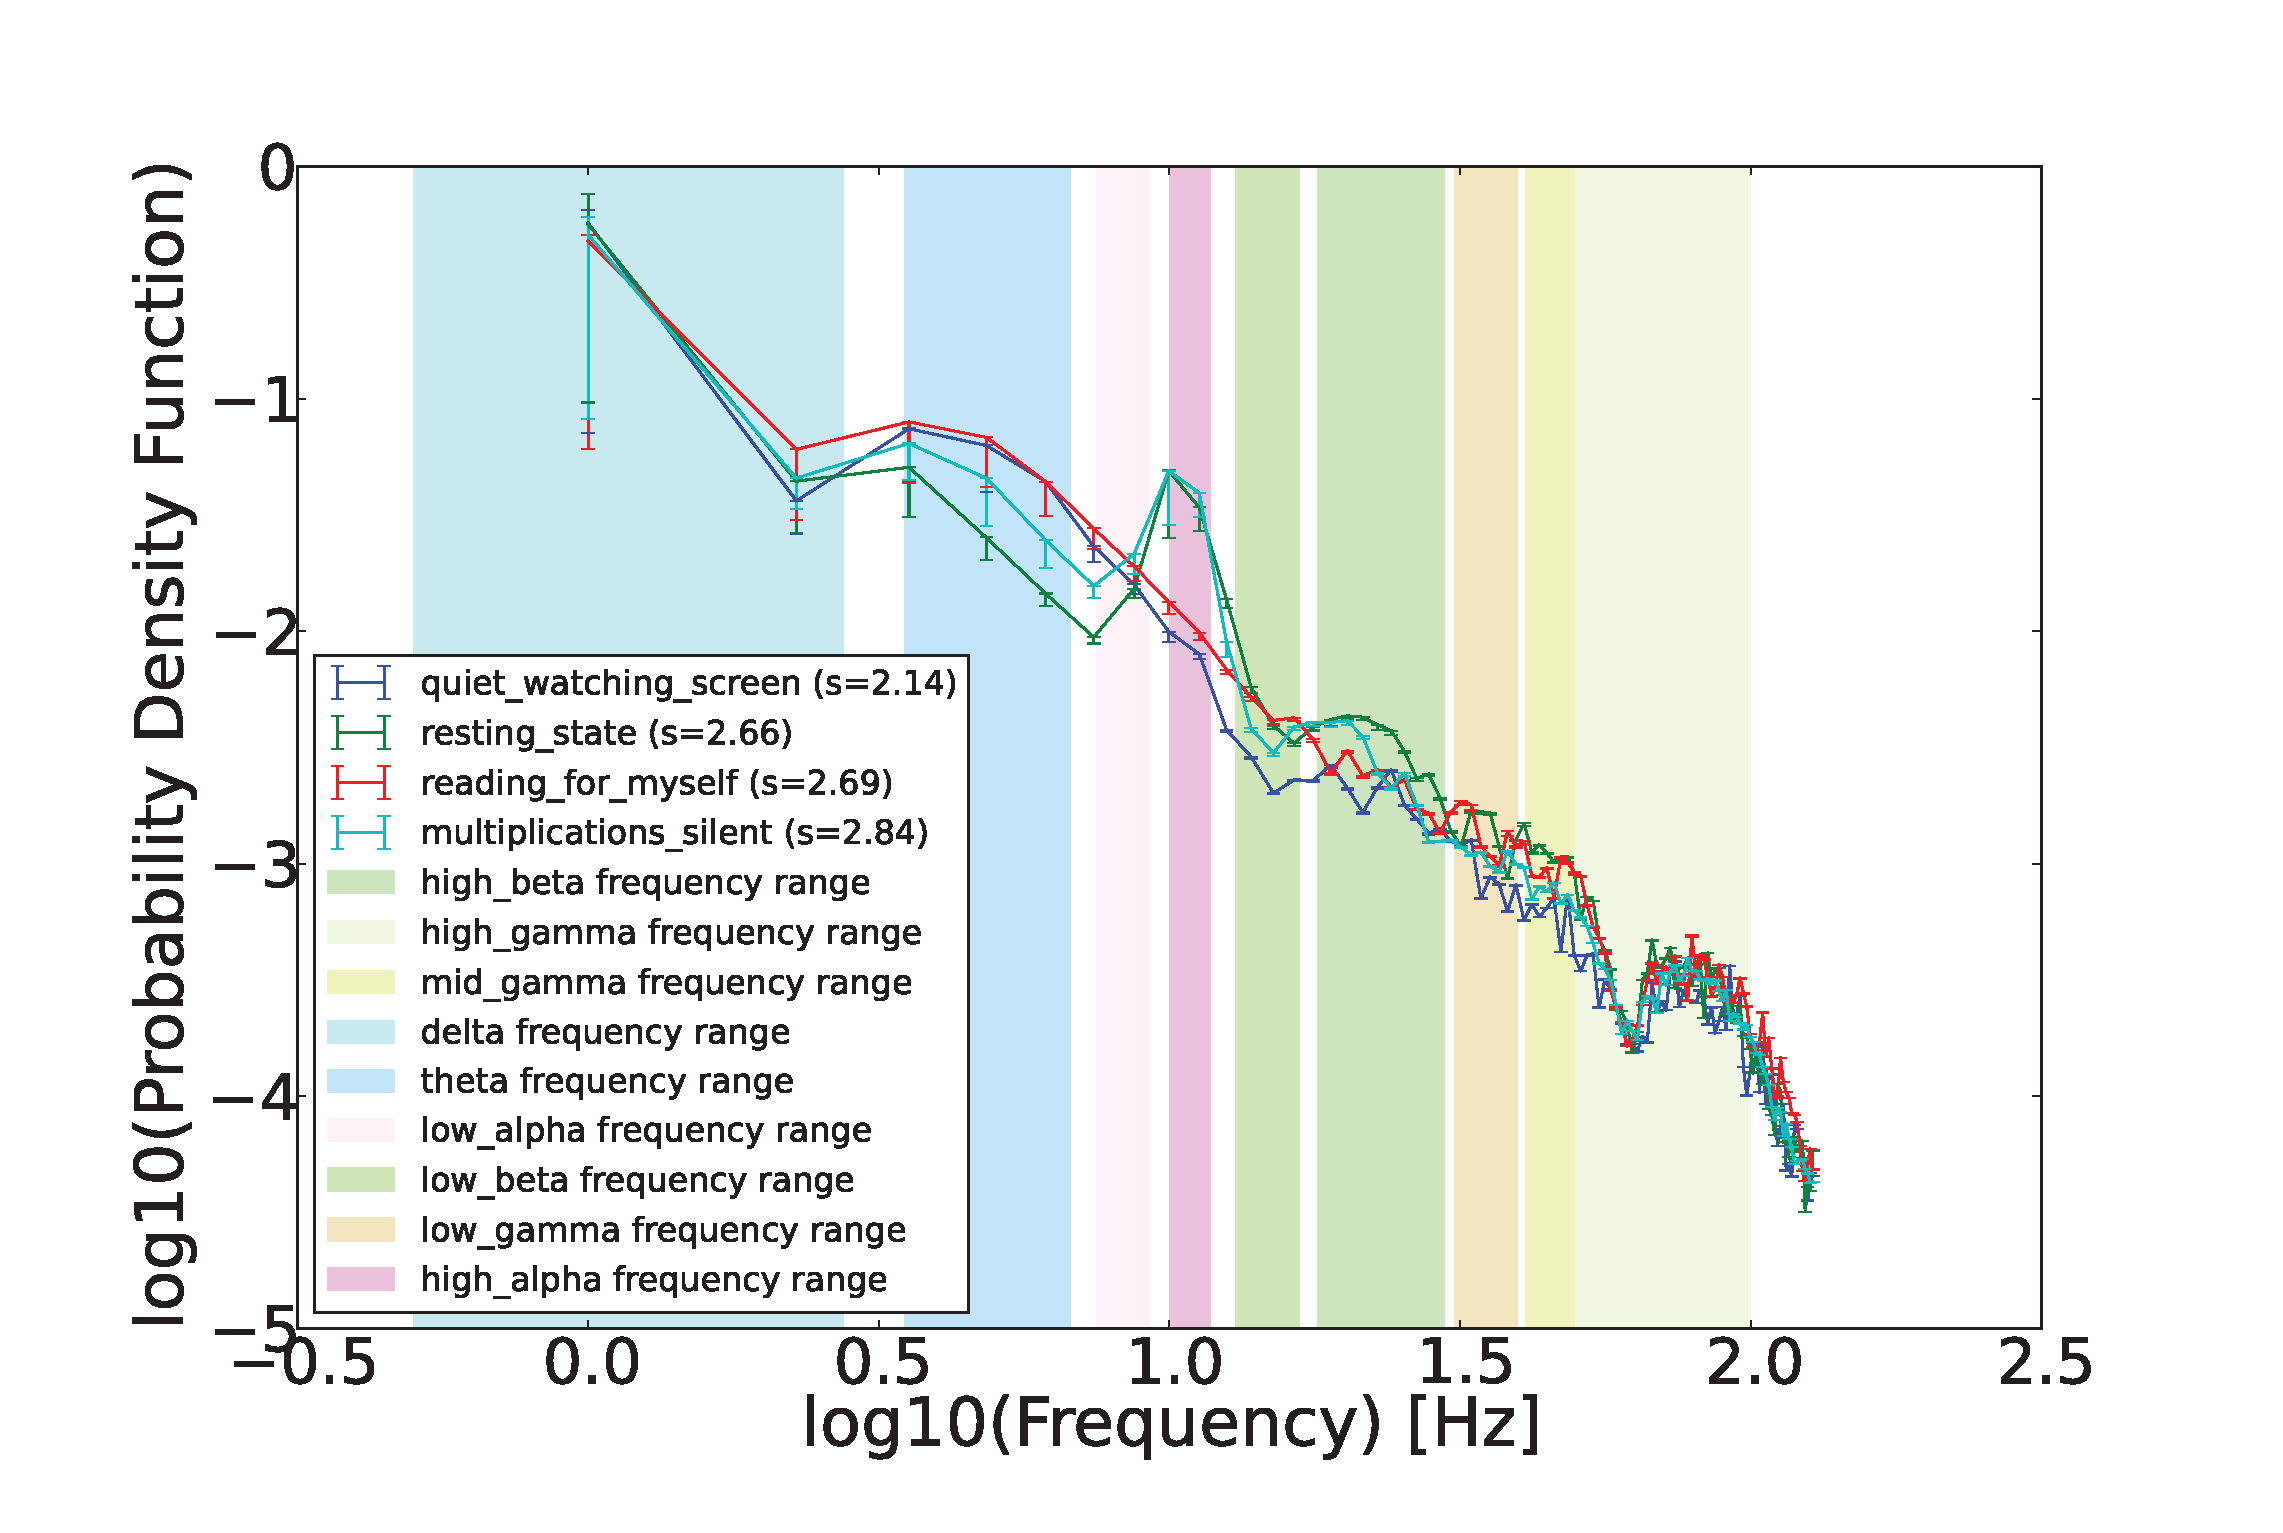
\includegraphics[width=1.1\columnwidth]{../figures/compareArtifacts.eps}
%\caption{Show the difference between resting state, being passive in front of a screen, and actively reading a text, in double logarithmic scale.}
%\label{fig:pspectrum}
%\end{figure}

%Figure \ref{fig:pspectrum} shows the heavy-tailed distribution of the power spectrum density, approximately a straight line in double logarithmic scale, which corresponds to current understanding of the pink noise nature of brain synchronization, $pdf(f) \sim 1/f^{\mu+1}$, with $f$ the frequency and $\mu \approx 1$ \cite{pink noise brain}.

\subsection{RSVP rate control mechanism}
With the normalized entropy $S_{norm}$, we have the most compact measure (i.e., a scalar) of brain state changes over a short period, as a result of the normalization (\ref{eq:Snormalized}). Although it is a rough {\it compressed} measure it captures all systematic changes of brain wave modulations (perturbations are considered to occur ranfomly). We shall now see how $S_{norm}$ controls the RSVP rate. 

We define $X = X(t)$ the presentation duration for each word. At each iteration, X is updated according to,

\begin{equation}
X(t+\Delta t) = X(t) \left[1 + \alpha \cdot S_{norm}(t)\right],
\label{eq:RateChange}
\end{equation}

with $S_{norm}$, the normalized entropy, continually updated according to (\ref{eq:Snormalized}), $\alpha$ is a small fixed parameter which determines the negative (resp. positive) incremental influence of $S_{norm}$ on $X(t)$. If $\alpha < 0$ and $S_{norm} > 0$, the RSVP rate decreases. Conversely, if $\alpha > 0$ and $S_{norm} > 0$, then the RSVP rate increases. Here, $|\alpha|$ is set to 0.005. We shall determine what sign of $\alpha$ is most convenient to users. If the median value of the EEG signal is superior to $150\mu v$, the measure of entropy $S$ is dropped, and the rate $X(t)$ is not updated. Separating sentences and paragraphs with small pauses is crucial to let subjects gain better understanding of the whole text \cite{}. After each sentence (resp. paragraph), we added the equivalent time of two (resp. four) words. For example, if the current rate is 150ms/word, then a pause of 300ms is used as a break between two sentences. 

Figure \ref{fig:apparatus} summarizes the apparatus and its step-by-step functioning: (i) the EEG signal is recorded, (ii)  processed online every quarter second  to obtain a power spectrum density, which is in turn (iii) represented by the normalized entropy  $S_{norm}$; (iv) depending on the values of parameter $\alpha$ and the random variable $S_{norm}$, the {\it brain speed reader} will change the RSVP rate. $X(t=0)$ is set to $125$ ms/word, which has been determined to be the comfort zone for RSVP reading \cite{kujala2007phase}.

\begin{figure}[!h]
\centering
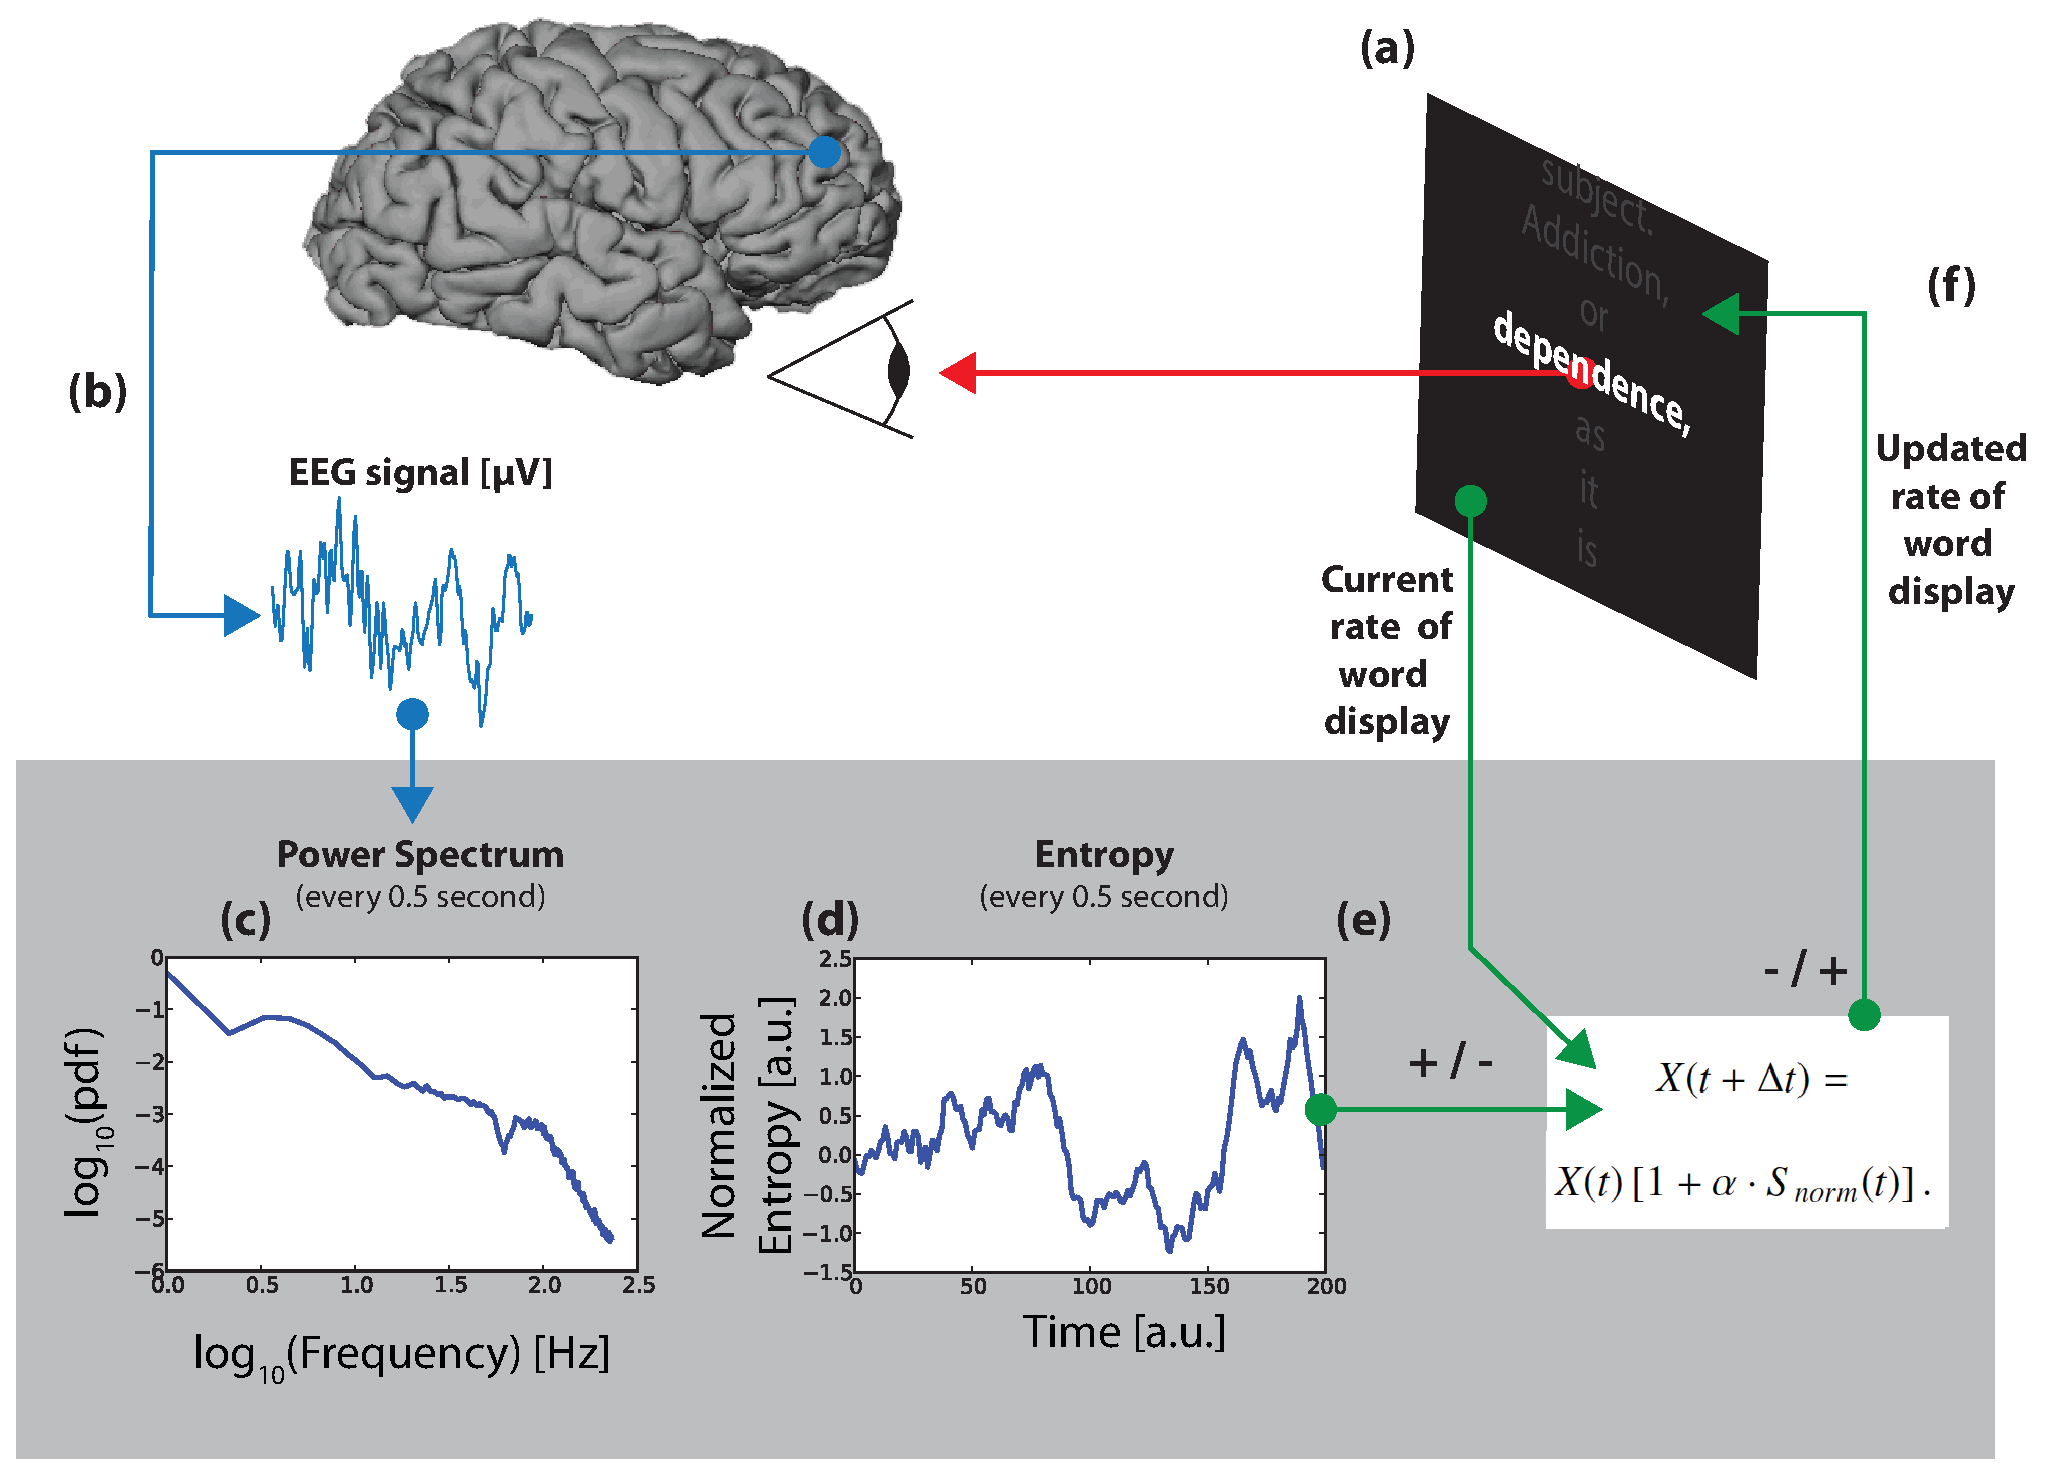
\includegraphics[width=0.9\columnwidth]{../figures2/apparatus.eps}
\caption{Brain speed-reader apparatus: {\bf (a)} Words are displayed and read one after the other at a given rate. {\bf (b)} the EEG signal is recorded through a consumer grade device (here the {\it Neurosky Mindwave}). {\bf (c)} The EEG signal is turned every 0.5 seconds into a power spectrum through a Fourier transform, {\bf (d)} the characteristics of the power spectrum are compressed into a single value characteristic entropy $s$ value. {\bf (e)} A new rate of word display is updated by taking into its current value and $s$. {\bf (f)} The rate of word display is updated accordingly.}
\label{fig:apparatus}
\end{figure}


\subsection{RSVP rate self-regulation}
Self-regulation neurofeedback is not granted to everyone, and we expect that some users may experience difficulty to achieve it. We therefore define a {\it stability} threshold, which measure is aimed at minimizing the ratio of the square formed by the two most extreme rates ($r_M$ for maximum rate and $r_m$ for the minimum rate), their time coordinates (resp. $k_{r_M}$ and  $k_{r_m}$) and by the number of words as the denominator. Although quite {\it ad-hoc}, this definition of stability encompasses transient rate changes, in particular those occurring when the brain speed reader starts as it takes some time for users to achieve self-regulation (see Figure \ref{fig:stability} for an illustration). By visual assessment, we consider that self-regulation is achieved for $stability < 2$ , although $stability$ is a continuous variable and the smaller its value, the better self-regulation. If the user reaches the upper or lower boundary (resp. $r_M = 30$  and $r_m = 175$ ms/word), then stability is arbitrarily set to 5.

\begin{equation}
stability = (r_M - r_m) \frac{|k_{r_M} - k_{r_m}|}{N} < 2
\label{eq:stability}
\end{equation}

\begin{figure}[!h]
\centering
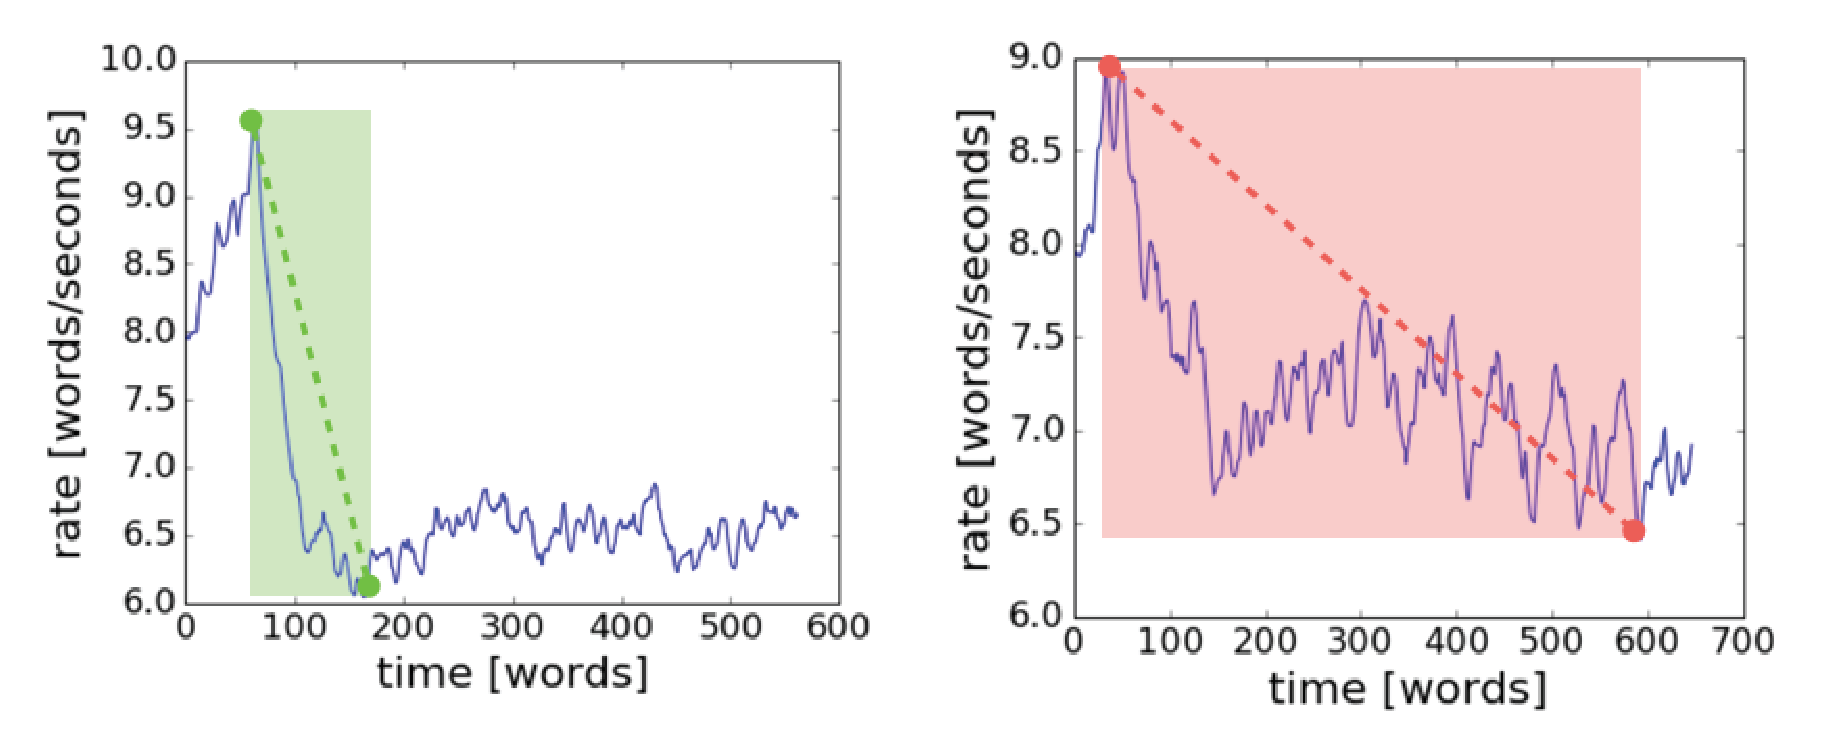
\includegraphics[width=0.9\columnwidth]{../figures2/stability_lowres.eps}
\caption{stability}
\label{fig:stability}
\end{figure}